\documentclass[12pt]{article}
\setlength\parindent{0pt}
\usepackage{fullpage}
\usepackage{graphicx}
\usepackage{amsmath}
\setlength{\parskip}{4mm}
\def\LL{\left\langle}   % left angle bracket
\def\RR{\right\rangle}  % right angle bracket
\def\LP{\left(}         % left parenthesis
\def\RP{\right)}        % right parenthesis
\def\LB{\left\{}        % left curly bracket
\def\RB{\right\}}       % right curly bracket
\def\PAR#1#2{ {{\partial #1}\over{\partial #2}} }
\def\PARTWO#1#2{ {{\partial^2 #1}\over{\partial #2}^2} }
\def\PARTWOMIX#1#2#3{ {{\partial^2 #1}\over{\partial #2 \partial #3}} }
\newcommand{\BE}{\begin{displaymath}}
\newcommand{\EE}{\end{displaymath}}
\newcommand{\BC}{\begin{center}}
\newcommand{\EC}{\end{center}}
\newcommand{\BNE}{\begin{equation}}
\newcommand{\ENE}{\end{equation}}
\newcommand{\BEA}{\begin{eqnarray}}
\newcommand{\EEA}{\nonumber\end{eqnarray}}
\newcommand{\EL}{\nonumber\\}
\newcommand{\la}[1]{\label{#1}}
\newcommand{\ie}{{\em i.e.\ }}
\newcommand{\eg}{{\em e.\,g.\ }}
\newcommand{\cf}{cf.\ }
\newcommand{\etc}{etc.\ }
\newcommand{\Tr}{{\rm tr}}
\newcommand{\etal}{{\it et al.}}
\newcommand{\OL}[1]{\overline{#1}\ } % overline
\newcommand{\OLL}[1]{\overline{\overline{#1}}\ } % double overline
\newcommand{\OON}{\frac{1}{N}} % "one over N"
\newcommand{\OOX}[1]{\frac{1}{#1}} % "one over X"



\begin{document}
\Large
\centerline{\sc{Homework 8}}
\normalsize
\centerline{\sc{Due Friday, 22 April, by the end of the day}}

The main part of HW8 is to redo Exam 3. (Anyone who earned 80\% or better on Exam 3 is exempt from this, and will get full credit for those questions.) See the link on the main website for the PDF.

{\it A note:} We will be liberal with extensions {\bf only until Monday} for this homework set. If you need an extension until Monday, please ask. 


There are two other exercises I'd like you to do; they are in this document.


\begin{enumerate}
	\item   A castle's drawbridge consists of a heavy wooden plank that can be opened or closed using a rope, as shown below:
	
	\begin{minipage}{0.5\textwidth}
		The rope is attached to the door 4/5 of the way down its length; the left side of the plank is attached to a hinge
		in the ground.
		The bridge is left in a partially-raised state by a careless sentry. It makes an angle of $30^\circ$ with the horizontal; the rope that supports it is perpendicular to the
		bridge.
	\end{minipage}
	\begin{minipage}{0.5\textwidth}
		\begin{center}
			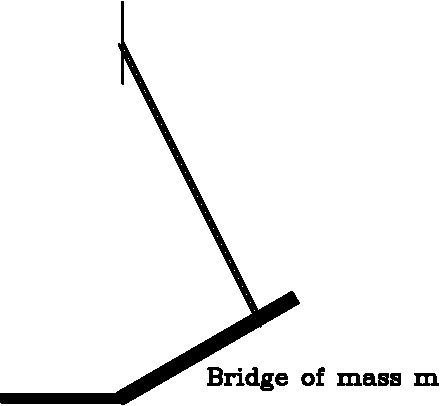
\includegraphics[width=0.6\textwidth]{door-crop.pdf}
		\end{center}
		
	\end{minipage}
	\medskip
	
	If the mass of the door is $m$, calculate the tension $T$ in the rope in terms of $\theta$, $m$, and $g$.
	
	
	\bigskip
	\bigskip
	
	
	\newpage
	\item 
	\textit{(This is an old exam problem.)} A meter stick is elevated at a $\theta=30^\circ$ angle. A spool consists of a cylinder of radius 2 cm with two disks affixed on either end; the disks have a 
	radius of 10 cm. The cylinder is very light; you may assume all of the mass of the spool is in the disks. The spool is placed at the top of the meter stick
	so that the cylinder is touching the stick; when it is released, it rolls without slipping to the bottom. \it (The moment of inertia of a disk is $\frac{1}{2}mr^2)$. \rm
	
	In this problem, you will calculate the speed of the spool at the bottom. 
	
	\small
	
	{\bf Rules for this problem:} You may solve this problem in either symbols or numbers. 
	If you use symbols, you must tell me the physical values of each symbol that you use (for instance: ``$r=2$ cm''). If you use numbers, you {\it must} retain the
	units (i.e. write ``10 cm'', not ``10''.)
	
	\normalsize
	
	\begin{minipage}{0.5\textwidth}
		\BC
		\it (Side view)
		
		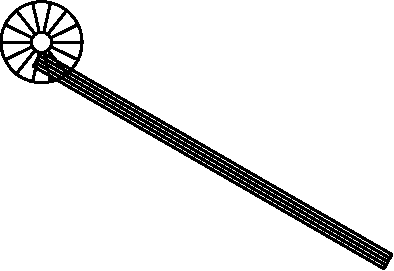
\includegraphics[width=0.8\textwidth]{sideview-crop.pdf}
		\EC
	\end{minipage}
	\begin{minipage}{0.5\textwidth}
		\BC
		\it (Rear view)
		
		\vspace{1cm}
		
		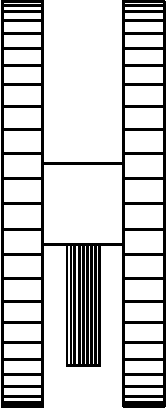
\includegraphics[width=0.2\textwidth]{rearview-crop.pdf}
		\EC
	\end{minipage}
	

	
	a) What is the relation between the spool's translational velocity $v$ and its angular velocity $\omega$? 
	

	b) Construct an equation showing the conservation of energy as the spool rolls down the slope. What sorts of energy does it have at the top? What about the bottom?
	
	c) Calculate the velocity of the spool at the bottom. Remember, if you use variables, you must tell me what number each symbol represents!
	
	
	
\end{enumerate}

\end{document}



